\section{为什么选择 Keras?}
在如今无数深度学习框架中,为什么要使用 Keras 而非其他?以下是 Keras与现有替代品的一些比较。


\subsection{Keras优先考虑开发人员的经验}

\begin{itemize}
\item
  Keras 是为人类而非机器设计的
  API。\href{https://blog.keras.io/user-experience-design-for-apis.html}{Keras
  遵循减少认知困难的最佳实践}: 它提供一致且简单的
  API,它将常见用例所需的用户操作数量降至最低,并且在用户错误时提供清晰和可操作的反馈。
\item
  这使 Keras 易于学习和使用。作为 Keras
  用户,你的工作效率更高,能够比竞争对手更快地尝试更多创意,从而\href{https://www.quora.com/Why-has-Keras-been-so-successful-lately-at-Kaggle-competitions}{帮助你赢得机器学习竞赛}。
\item
  这种易用性并不以降低灵活性为代价:因为 Keras
  与底层深度学习语言(特别是
  TensorFlow)集成在一起,所以它可以让你实现任何你可以用基础语言编写的东西。特别是,\texttt{tf.keras}
  作为 Keras API 可以与 TensorFlow 工作流无缝集成。
\end{itemize}


\subsection{Keras被工业界和学术界广泛采用}

\begin{figure}[h]
\begin{center}
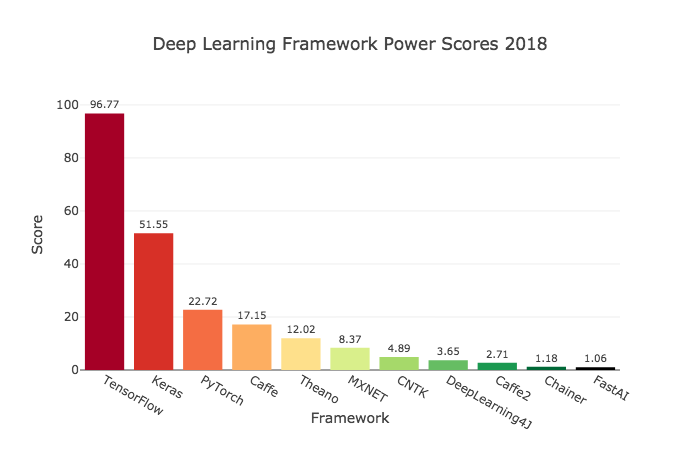
\includegraphics[width=\textwidth]{figure/framework_rank.png}
\end{center}
\caption{Deep learning 框架排名,由 Jeff Hale 基于 7 个分类的 11 个数据源计算得出}
\end{figure}

截至 2018 年中期,Keras 拥有超过 250,000 名个人用户。与其他任何深度学习框架相比,Keras 在行业和研究领域的应用率更高(除 TensorFlow 之外,且 Keras API 是 TensorFlow 的官方前端,通过 \texttt{tf.keras} 模块使用)。

您已经不断与使用 Keras 构建的功能进行交互 - 它在 Netflix, Uber, Yelp,
Instacart, Zocdoc, Square
等众多网站上使用。它尤其受以深度学习作为产品核心的创业公司的欢迎。

Keras也是深度学习研究人员的最爱,在上载到预印本服务器
\href{https://arxiv.org/archive/cs}{arXiv.org}
的科学论文中被提及的次数位居第二。Keras
还被大型科学组织的研究人员采用,特别是 CERN 和 NASA。




\subsection{Keras 可以轻松将模型转化为产品}

与任何其他深度学习框架相比,你的 Keras 模型可以轻松部署在更广泛的平台上:

\begin{itemize}
\tightlist
\item
  在 iOS 上,通过
  \href{https://developer.apple.com/documentation/coreml}{Apple's
  CoreML}(苹果为 Keras 提供官方支持)。这里有一个\href{https://www.pyimagesearch.com/2018/04/23/running-keras-models-on-ios-with-coreml/}{教程}。
\item
  在安卓 上,通过 TensorFlow Android
  runtime,例如:\href{https://medium.com/@timanglade/how-hbos-silicon-valley-built-not-hotdog-with-mobile-tensorflow-keras-react-native-ef03260747f3}{Not
  Hotdog app}。
\item
  在浏览器上,通过 GPU 加速的 JavaScript
  运行时,例如:\href{https://transcranial.github.io/keras-js/\#/}{Keras.js}
  和 \href{https://mil-tokyo.github.io/webdnn/}{WebDNN}。
\item
  在 Google Cloud 上,通过
  \href{https://www.tensorflow.org/serving/}{TensorFlow-Serving}。
\item
  \href{https://blog.keras.io/building-a-simple-keras-deep-learning-rest-api.html}{在 Python 网页应用后端(比如 Flask app)中}。
\item
  在 JVM,通过
  \href{https://deeplearning4j.org/model-import-keras}{SkyMind 提供的
  DL4J 模型导入}。
\item
  在 Raspberry Pi 树莓派上。
\end{itemize}


\subsection{Keras
支持多个后端引擎,并且不会将你锁定到一个生态系统中}\label{keras-ux652fux6301ux591aux4e2aux540eux7aefux5f15ux64ceux5e76ux4e14ux4e0dux4f1aux5c06ux4f60ux9501ux5b9aux5230ux4e00ux4e2aux751fux6001ux7cfbux7edfux4e2d}

你的 Keras
模型可以基于不同的\hyperref[keras-backend]{深度学习后端}开发。重要的是,任何仅利用内置层构建的
Keras
模型,都可以在所有这些后端中移植:用一种后端训练模型,再将它载入另一种后端中(比如为了发布)。支持的后端有:

\begin{itemize}
\tightlist
\item
  谷歌的 TensorFlow 后端
\item
  微软的 CNTK 后端
\item
  Theano 后端
\end{itemize}

亚马逊也正在为 Keras 开发 MXNet 后端。

如此一来,你的 Keras 模型可以在 CPU 之外的不同硬件平台上训练:

\begin{itemize}
\tightlist
\item
  \href{https://developer.nvidia.com/deep-learning}{NVIDIA GPU}。
\item
  \href{https://cloud.google.com/tpu/}{Google TPU},通过 TensorFlow
  后端和 Google Cloud。
\item
  OpenGL 支持的 GPU, 比如 AMD, 通过
  \href{https://github.com/plaidml/plaidml}{PlaidML Keras 后端}。
\end{itemize}


\subsection{Keras 拥有强大的多 GPU
和分布式训练支持}

\begin{itemize}
\tightlist
\item
  Keras \hyperref[multi-gpu-model]{内置对多 GPU
  数据并行的支持}。
\item
  优步的 \href{https://github.com/uber/horovod}{Horovod} 对 Keras
  模型有第一流的支持。
\item
  Keras
  模型\href{https://www.tensorflow.org/versions/master/api_docs/python/tf/keras/estimator/model_to_estimator}{可以被转换为
  TensorFlow 估计器}并在
  \href{https://cloud.google.com/solutions/running-distributed-tensorflow-on-compute-engine}{Google
  Cloud 的 GPU 集群}上训练。
\item
  Keras 可以在 Spark(通过 CERN 的
  \href{https://github.com/cerndb/dist-keras}{Dist-Keras})和~\href{https://github.com/maxpumperla/elephas}{Elephas}
  上运行。
\end{itemize}


\subsection{Keras
的发展得到深度学习生态系统中的关键公司的支持}\label{keras-ux7684ux53d1ux5c55ux5f97ux5230ux6df1ux5ea6ux5b66ux4e60ux751fux6001ux7cfbux7edfux4e2dux7684ux5173ux952eux516cux53f8ux7684ux652fux6301}

Keras 的开发主要由谷歌支持,Keras API 以 \texttt{tf.keras} 的形式包装在
TensorFlow 中。此外,微软维护着 Keras 的 CNTK 后端。亚马逊 AWS 正在开发
MXNet 支持。其他提供支持的公司包括 NVIDIA、优步、苹果(通过 CoreML)等。

\newpage
